\section{Akvizicija zvuka}

Podsustav za akviziciju zvuka je usko vezan uz platformu na kojoj
je sustav implementiran zbog toga što je zadužen za komunikaciju 
sa sustavom koji prikuplja stvarne signale sa senzora (mikrofona).
ESP32 Lyrat Development Board \cite{lyrat}, na kojem je sustav
implementiran, na sebi ima već ugrađen mikrofon i audio kodek
s kojim je moguće komunicirati putem I2S protokola. Na slici
\ref{pic:esp} prikazan je blok dijagram ESP32 razvojne platforme.

\begin{figure}[htb]
    \centering
    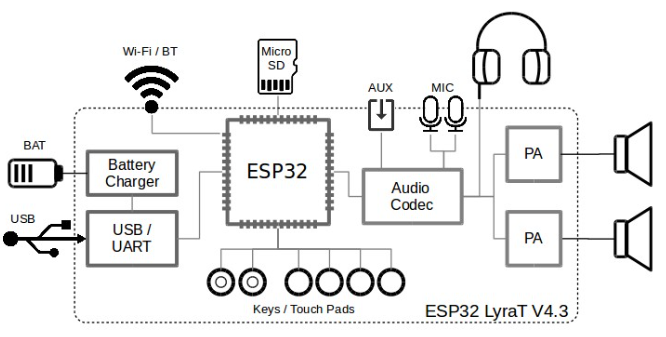
\includegraphics[width=0.6\linewidth]{Chapters/struktura_sustava/akvizicija/lyrat.png} 
    \caption{ESP32 Lyrat \cite{lyrat}}
    \label{pic:esp}
\end{figure}

Najvažniji dio razvojne platforme je upravo ESP32-WROVER-E mikrokontroler
na kojem je cjelopukni sustav za prepoznavanje govnornih naredbi 
implementiran. Upravo on je zadužen za komunikaciju s ES8388 
audio kodekom \cite{es8388}. MEMS mikrofon
akvizira zvučni signal kojeg audio kodek digitalizira i kojeg je onda
moguće 